\section{Hall Sensor}
For the measurement of the homogeneity of the field the data points were plotted in figure \ref{Homogen}. It can be seen clearly that after a depth of $7$\,mm inside the field no change is noticeable so our field is uniform at this point.
\begin{figure}[ht]
	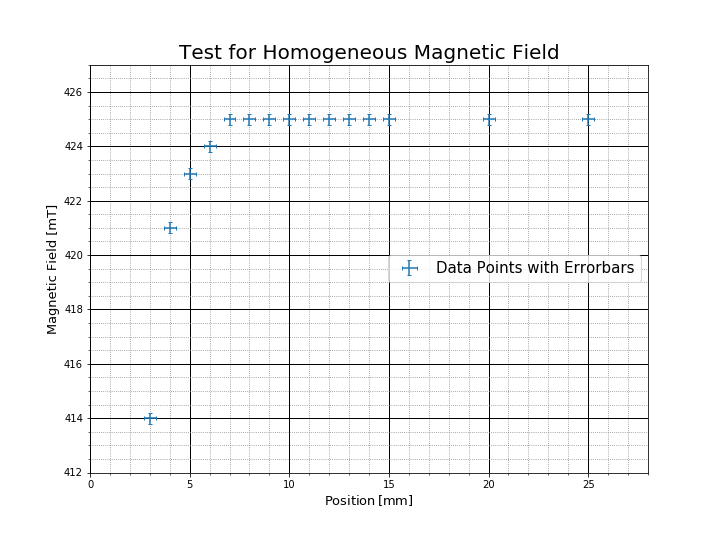
\includegraphics[scale=0.5]{Bild/Hallsonde}
	\centering
	\caption[Uniformity of the Magnetic Field]{The strength of the magnetic field depending on the depth inside the field.}
	\label{Homogen}
\end{figure}\\
Since the first Hall sensor was destroyed during the experiment another one had to be used. This one showed a change in the magnetic field depending on the time it was inside the field. To increase the accuracy of the experiment this change was measured once with the sawtooth and once without it. These two can be seen in figure \ref{Hallsonde1} and \ref{Hallsonde2}.
\begin{figure}[ht]
	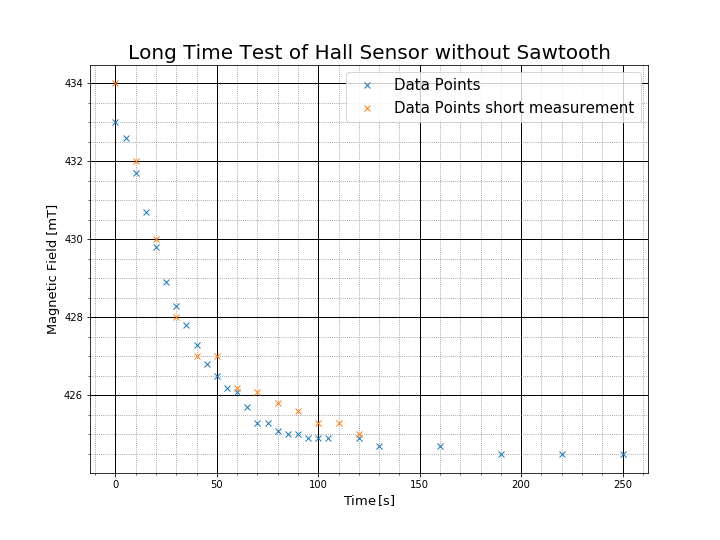
\includegraphics[scale=0.5]{Bild/Hallsonde1}
	\centering
	\caption[Hall Sensor without Sawtooth]{Measurement of the magnetic field depending of the time inside the field with the sawtooth shaped signal. The errors for the data points were to small to make them clearly visible.}
	\label{Hallsonde1}
\end{figure}
\begin{figure}[ht]
	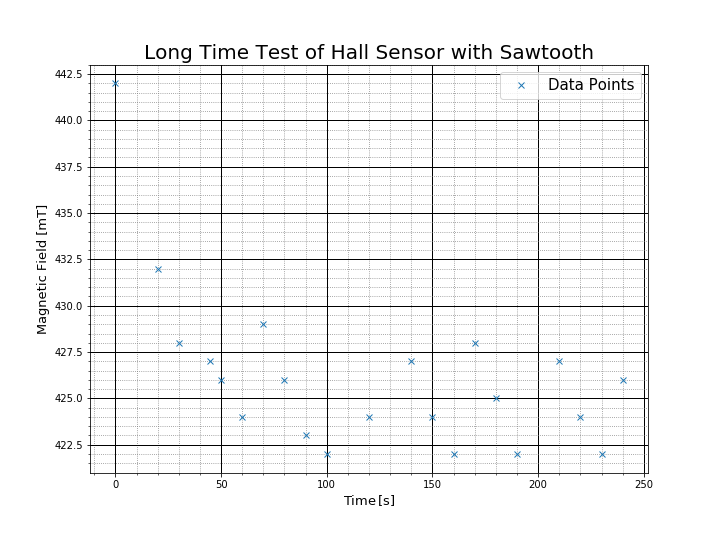
\includegraphics[scale=0.5]{Bild/Hallsonde2}
	\centering
	\caption[Hall Sensor with Sawtooth]{Measurement of the magnetic field depending of the time inside the field without the sawtooth shaped signal. Here two measurements were made one in orange the other one in blue. The errors for the data points were to small to make them clearly visible.}
	\label{Hallsonde2}
\end{figure}
It is clearly visible that time has an impact on the measurement. In fig.\ref{Hallsonde1} we the that for once the change from the sawtooth which slowly decreases the magnetic field and than increases it suddenly. In fig.\ref{Hallsonde2} the saturation of after a certain time is seen. It is very likely that the temperature inside point of measurement changes the properties of the Hall sensor. With that it is not clear which is the correct magnetic field. The one at the saturation or the beginning when the sensor is close the room temperature. Inside the manual of the electro magnets a hysteresis curve was found giving the magnetic field depending on the amperage.\cite{Electromagnet} Since the amperage during the measurement was at $3.41$\,A the magnetic field strength should be around $415$,mT. This value is not very precise since the curve could have changed over time but it clearly shows, that the saturation value is more precise. Since the upper one was used for the measurements, a large systematic error has to be expected for all measurements taken with the new Hall sensor.